\subsection{Máquina de estados algorítmica programable}

Un procesador puede ser visto como una máquina de estados programable como la que se muestra en la figura \ref{processor_block_diagram}. En ella podemos ver un camino de datos fijo (bloques naranja) formado por un banco de registros, una unidad lógico-aritmética; el banco de registros está compuesto por varios registros de propósito general que pueden ser utilizados para almacenar las variables de un determinado algoritmo, la salida de este banco está conectada con el bloque lógico aritmético y permite pasar dos parámetros al mismo tiempo para realizar cualquier tipo de operación, la salida de la unidad lógico aritmética se realimenta al banco de registros para almacenar el resultado. Con esta arquitectura se pierde velocidad de ejecución ya que todas las operaciones deben ser realizadas en la unidad lógico-aritmética, pero se gana flexibilidad al poder ejecutar varios algoritmos con el mismo camino de datos.

\begin{figure}[htpb]
  \centering
  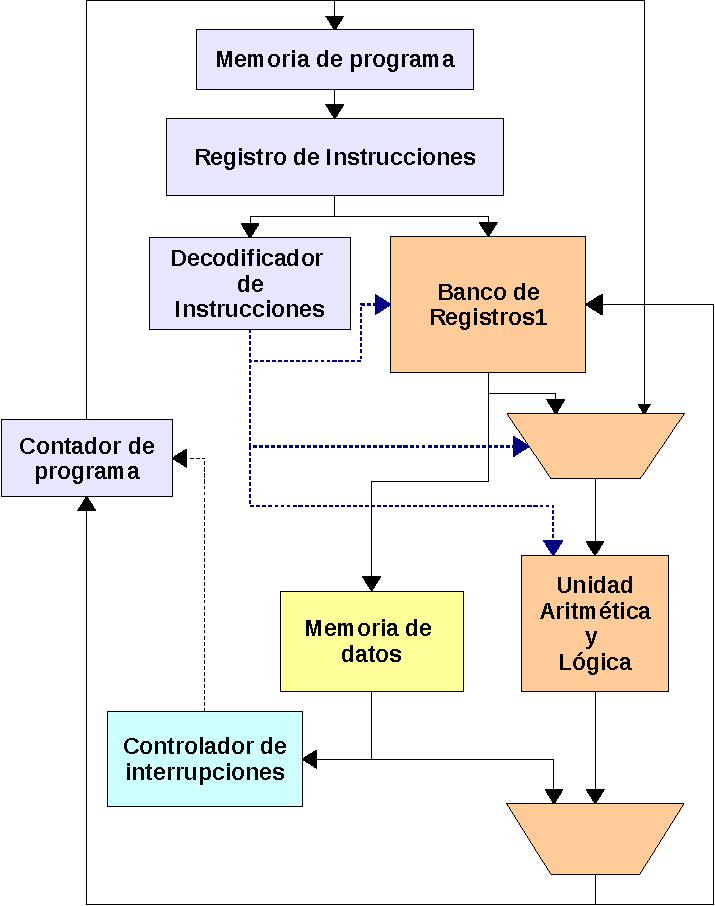
\includegraphics[width=6.879cm,height=5.08cm]{./images/processor_block_diagram.pdf}
  \caption{Diagrama de bloques para una ASM programable.} \label{processor_block_diagram}
\end{figure}


Para que este camino de datos pueda ejecutar diferentes algoritmos es necesario incluir módulos que se encarguen de (bloques de color azul en la figura \ref{processor_block_diagram}): almacenar las instrucciones que implementan el algoritmo y ejecutar estas instrucciones controlando las señales del camino de datos. La \textit{memoria de programa} almacena las instrucciones que deben ser ejecutadas para obtener la funcionalidad deseada; las instrucciones que se puedan ejecutar depende del diseño del procesador y se reciben el nombre de \textit{set de instrucciones}, el programador debe utilizar este conjunto de instrucciones para implementar la funcionalidad deseada.

El \textit{contador de programa} (PC) contiene la dirección de la instrucción que se está ejecutando en un instante determinado, esto, debido a que controla el bus de direcciones de la memoria de programa. Una vez se ejecuta una instrucción el valor del contador de programa aumenta en 1 para tomar las siguiente instrucción. La instrucción señalada por el contador de programa es almacenada en el \textit{registro de instrucciones} durante todo el ciclo de ejecución (de la instrucción), el \textit{decodificador de instrucciones} identifica la instrucción y controla las señales del camino de datos para ejecutar las operaciones asociadas a ella. Las instrucciones que implementan el algoritmo deben almacenarse de forma ascendente en la memoria de programa de tal forma que para ejecutar el algoritmo solo sea necesario aumentar el valor del \textit{contador de programa}, capturar, decodificar y ejecutar la instrucción correspondiente en la memoria de programa.


Si el valor del contador de programa no se pudiera modificar y solo pudiera aumentarse de uno en uno, el flujo del programa sería continuo, sin saltos; los saltos son necesarios para implementar bloques de decisión (\textit{if, case}) y ciclos (\textit{for, while}); para permitir el uso de bloques de decisión y ciclos se debe incluir un mecanismo que permita modificar el valor del contador de programa, para ello, el valor del contador de programa tiene una entrada al bloque lógico-aritmético y la salida de este bloque puede modificar el valor del contador de programa; para aclarar esto consideremos la implementación de un bloque de decisión, si la condición se cumple entonces debemos ejecutar un grupo de instrucciones localizadas en una posición cercana, por lo que es necesario hacer un salto relativo a la posición actual del contador de programa, esto es, \textit{PC = PC + val}, para hacer esta operación debemos: pasar el valor del PC y el valor \textit{val} a dos registros del banco de registros; pasar el 
contenido de estos dos registros al bloque lógico-aritmético para ser sumados; almacenar el resultado en el PC.


